
%(BEGIN_QUESTION)
% Copyright 2010, Tony R. Kuphaldt, released under the Creative Commons Attribution License (v 1.0)
% This means you may do almost anything with this work of mine, so long as you give me proper credit

Suppose an Allen-Bradley PLC controls the starting and stopping of a conveyor belt, using a timer to sound an audible warning siren for 5 seconds before the conveyor belt starts up (to warn people before the belt begins to move):

$$\includegraphics[width=15.5cm]{i02259x01.eps}$$

Determine the necessary contact connections (form-A or form-B) on the real-life Start, Stop, and emergency Pull-Cable switches to complement the virtual contact types in the PLC program.

\vskip 10pt

Start switch = form-A {\it or} form-B?

\vskip 10pt

Stop switch = form-A {\it or} form-B?

\vskip 10pt

Pull-Cable switch = form-A {\it or} form-B?

\vskip 20pt \vbox{\hrule \hbox{\strut \vrule{} {\bf Suggestions for Socratic discussion} \vrule} \hrule}

\begin{itemize}
\item{} How could you modify this program so that the operator has to hold the ``Start'' pushbutton switch actuated for the duration of the warning siren before the motor would start (i.e. everything would simply stop if the operator only {\it momentarily} pressed the ``Start'' button)?
\item{} Suppose a technician decides to use the {\it force} utility in the PLC to force bit {\tt B3:0/0} to a ``0'' state in order to test the warning siren's operation without actually starting up the conveyor belt.  Explain what is flawed with this testing strategy, and identify a better approach.
\item{} How will this system behave if the pull-cable switch fails open?
\item{} How will this system behave if the stop switch fails shorted?
\end{itemize}

\underbar{file i02259}
%(END_QUESTION)





%(BEGIN_ANSWER)


%(END_ANSWER)





%(BEGIN_NOTES)

Start switch = {\bf form-A} (normally-open)

\vskip 10pt

Stop switch = {\bf form-B} (normally-closed)

\vskip 10pt

Pull-Cable switch = {\bf form-A} (normally-open)

%INDEX% PLC, relating I/O status to virtual elements 

%(END_NOTES)


